\def\layersep{2.5cm}

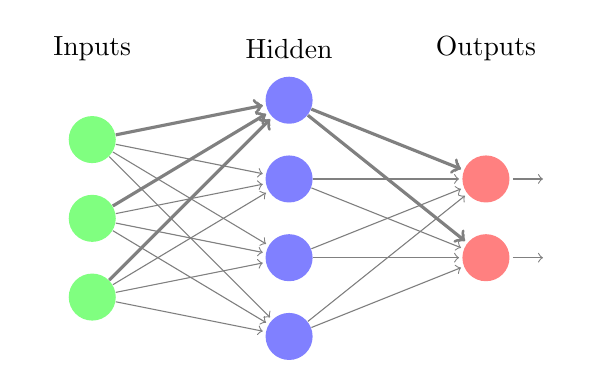
\begin{tikzpicture}[shorten >=1pt,->,draw=black!50, node distance=\layersep]
    \tikzstyle{every pin edge}=[<-,shorten <=1pt]
    \tikzstyle{neuron}=[circle,fill=black!25,minimum size=17pt,inner sep=0pt]
    \tikzstyle{input neuron}=[neuron, fill=green!50];
    \tikzstyle{output neuron}=[neuron, fill=red!50];
    \tikzstyle{hidden neuron}=[neuron, fill=blue!50];
    \tikzstyle{bias neuron}=[neuron, fill=yellow!50];
    \tikzstyle{annot} = [text width=4em, text centered]

    % Draw the input layer nodes.
    \foreach \name / \y in {1,...,3}
        \node[input neuron] (I-\name) at (0,-\y) {};

    % Draw the hidden layer nodes.
    \foreach \name / \y in {1,...,4}
        \path[yshift=0.5cm]
            node[hidden neuron] (H-\name) at (\layersep,-\y cm) {};

    % Draw the output layer nodes
    \node[output neuron,pin={[pin edge={->}]right:}, right of=H-2] (O-1) {};
    \node[output neuron,pin={[pin edge={->}]right:}, right of=H-3] (O-2) {};

    % Connect input layer with hidden layer.
    \foreach \source in {1,...,3}
        \foreach \dest in {1,...,4}
            \path (I-\source) edge (H-\dest);

    % Connect hidden layer with output layer.
    \foreach \source in {1,...,4}
        \path (H-\source) edge (O-1);

    \foreach \source in {1,...,4}
        \path (H-\source) edge (O-2);


    % Higlight path
    \foreach \source in {1,...,3}
        \draw[->,line width=0.4mm] (I-\source)--(H-1) node[pos=.6,above]{};

    \foreach \dest in {1,...,2}
        \draw[->,line width=0.4mm] (H-1)--(O-\dest) node[pos=.6,above]{};
    % Annotate the layers.
    \node[annot,above of=H-1, node distance=0.65cm] (hl) {Hidden};
    \node[annot,left of=hl] {Inputs};
    \node[annot,right of=hl] {Outputs};
\end{tikzpicture}